\documentclass{llncs}\usepackage[]{graphicx}\usepackage[]{color}
%% maxwidth is the original width if it is less than linewidth
%% otherwise use linewidth (to make sure the graphics do not exceed the margin)
\makeatletter
\def\maxwidth{ %
  \ifdim\Gin@nat@width>\linewidth
    \linewidth
  \else
    \Gin@nat@width
  \fi
}
\makeatother

\definecolor{fgcolor}{rgb}{0.345, 0.345, 0.345}
\newcommand{\hlnum}[1]{\textcolor[rgb]{0.686,0.059,0.569}{#1}}%
\newcommand{\hlstr}[1]{\textcolor[rgb]{0.192,0.494,0.8}{#1}}%
\newcommand{\hlcom}[1]{\textcolor[rgb]{0.678,0.584,0.686}{\textit{#1}}}%
\newcommand{\hlopt}[1]{\textcolor[rgb]{0,0,0}{#1}}%
\newcommand{\hlstd}[1]{\textcolor[rgb]{0.345,0.345,0.345}{#1}}%
\newcommand{\hlkwa}[1]{\textcolor[rgb]{0.161,0.373,0.58}{\textbf{#1}}}%
\newcommand{\hlkwb}[1]{\textcolor[rgb]{0.69,0.353,0.396}{#1}}%
\newcommand{\hlkwc}[1]{\textcolor[rgb]{0.333,0.667,0.333}{#1}}%
\newcommand{\hlkwd}[1]{\textcolor[rgb]{0.737,0.353,0.396}{\textbf{#1}}}%

\usepackage{framed}
\makeatletter
\newenvironment{kframe}{%
 \def\at@end@of@kframe{}%
 \ifinner\ifhmode%
  \def\at@end@of@kframe{\end{minipage}}%
  \begin{minipage}{\columnwidth}%
 \fi\fi%
 \def\FrameCommand##1{\hskip\@totalleftmargin \hskip-\fboxsep
 \colorbox{shadecolor}{##1}\hskip-\fboxsep
     % There is no \\@totalrightmargin, so:
     \hskip-\linewidth \hskip-\@totalleftmargin \hskip\columnwidth}%
 \MakeFramed {\advance\hsize-\width
   \@totalleftmargin\z@ \linewidth\hsize
   \@setminipage}}%
 {\par\unskip\endMakeFramed%
 \at@end@of@kframe}
\makeatother

\definecolor{shadecolor}{rgb}{.97, .97, .97}
\definecolor{messagecolor}{rgb}{0, 0, 0}
\definecolor{warningcolor}{rgb}{1, 0, 1}
\definecolor{errorcolor}{rgb}{1, 0, 0}
\newenvironment{knitrout}{}{} % an empty environment to be redefined in TeX

\usepackage{alltt}
\usepackage{listings}
\usepackage{moreverb}
\usepackage{inconsolata}



\IfFileExists{upquote.sty}{\usepackage{upquote}}{}
\begin{document}

\title{Problem Set 3}
\author{Thibault Doutre, ID : 26980469}
\institute{STAT 243 : Introduction to Statistical Computing}
\date{}
\maketitle
\bigbreak
\noindent
I worked on my own.

%%%%%%%%%%%%%%%%%%%%%%%%%%%%%%%%%%%%%%%%%%%%%%%%%%%%%%%%%%%
\section{Problem 1}
%%%%%%%%%%%%%%%%%%%%%%%%%%%%%%%%%%%%%%%%%%%%%%%%%%%%%%%%%%%%
Wilson et.al

About section 7, Defensive programming :

In R, how do we add assertion to programs ? Should we use the "print" function ? I am afraid that it will slow down the program if I use it in a for loop for example. 

About section 10, Collaborate :

Is pair programming widely used in the industry ?

%%%%%%%%%%%%%%%%%%%%%%%%%%%%%%%%%%%%%%%%%%%%%%%%%%%%%%%%%%%
\section{Problem 2}
%%%%%%%%%%%%%%%%%%%%%%%%%%%%%%%%%%%%%%%%%%%%%%%%%%%%%%%%%%%%
%%%%%%%%%%%%%%%%%%%%%%
\subsection{Extract URL}
%%%%%%%%%%%%%%%%%%%%%%
First, I load the necessary databases and store the link provided.
\begin{knitrout}
\definecolor{shadecolor}{rgb}{0.969, 0.969, 0.969}\color{fgcolor}\begin{kframe}
\begin{alltt}
\hlkwd{library}\hlstd{(XML)}
\hlkwd{library}\hlstd{(stringr)}
\hlstd{link}\hlkwb{=}\hlstr{"http://www.debates.org/index.php?page=debate-transcripts"}
\end{alltt}
\end{kframe}
\end{knitrout}
\noindent
Then, I create a function which takes the year of the debate and gives us:
\begin{itemize}
  \item The URL of the first debate
  \item The names of the candidates
\end{itemize}
\begin{knitrout}
\definecolor{shadecolor}{rgb}{0.969, 0.969, 0.969}\color{fgcolor}\begin{kframe}
\begin{alltt}
\hlstd{extract_URL_debate} \hlkwb{=} \hlkwa{function}\hlstd{(}\hlkwc{year}\hlstd{)\{}
  \hlcom{#Load HTML as a tree (with nodes)}
  \hlstd{doc}\hlkwb{=}\hlkwd{htmlTreeParse}\hlstd{(link)}
  \hlcom{#Extract body of the doc}
  \hlstd{root} \hlkwb{=} \hlkwd{xmlRoot}\hlstd{(doc)}
  \hlstd{body}\hlkwb{=} \hlkwd{xmlChildren}\hlstd{(root)}\hlopt{$}\hlstd{body}
  \hlcom{#Find the four debates of every year : Each element of the list }
  \hlcom{#corresponds to different year}
  \hlstd{debates_years}\hlkwb{=}\hlkwd{xpathApply}\hlstd{(body,} \hlstr{"//div/..//blockquote"}\hlstd{)}
  \hlcom{#Map the position of the list with the corresponding year}
  \hlstd{code_year}\hlkwb{=}\hlstd{(}\hlnum{2012}\hlopt{-}\hlstd{year)}\hlopt{/}\hlnum{4}\hlopt{+}\hlnum{1}
  \hlcom{#Find the 4 debates for the required year}
  \hlstd{debates_year}\hlkwb{=}\hlkwd{xpathApply}\hlstd{(debates_years[[code_year]],}\hlstr{"//a"}\hlstd{)}
  \hlcom{#Find description of each debate}
  \hlstd{description}\hlkwb{=}\hlkwd{sapply}\hlstd{(debates_year, xmlValue)}
  \hlcom{#Find the position of the First debate}
  \hlstd{no_debate}\hlkwb{=}\hlkwd{grep}\hlstd{(}\hlstr{"First"}\hlstd{,description)}
  \hlcom{#Extract president names from description}
  \hlstd{candidates_value}\hlkwb{=}\hlkwd{xmlValue}\hlstd{(debates_year[[no_debate]])}
  \hlstd{duo}\hlkwb{=}\hlkwd{str_extract}\hlstd{(}\hlkwd{as.character}\hlstd{(candidates_value),}
                  \hlstr{"[a-zA-z]+\textbackslash{}\textbackslash{}-[a-zA-z]+"}\hlstd{)}
  \hlstd{candidates}\hlkwb{=}\hlkwd{str_split}\hlstd{(duo,}\hlstr{"-"}\hlstd{)}
  \hlcom{#Extract and return URL}
  \hlkwd{return} \hlstd{(}\hlkwd{list}\hlstd{(}\hlkwc{URL}\hlstd{=}\hlkwd{xmlGetAttr}\hlstd{(debates_year[[no_debate]],}\hlstr{"href"}\hlstd{),}
               \hlkwc{Names}\hlstd{=}\hlkwd{toupper}\hlstd{(candidates[[}\hlnum{1}\hlstd{]])))}
\hlstd{\}}
\end{alltt}
\end{kframe}
\end{knitrout}
\noindent
For example, for the debate of 2012, we have :
\begin{knitrout}
\definecolor{shadecolor}{rgb}{0.969, 0.969, 0.969}\color{fgcolor}\begin{kframe}
\begin{alltt}
\hlkwd{extract_URL_debate}\hlstd{(}\hlnum{2012}\hlstd{)}
\end{alltt}
\begin{lstlisting}[basicstyle=\ttfamily,breaklines=true]
## $URL
## [1] "http://www.debates.org/index.php?page=october-3-2012-debate-transcript"
## 
## $Names
## [1] "OBAMA"  "ROMNEY"
\end{lstlisting}
\end{kframe}
\end{knitrout}
%%%%%%%%%%%%%%%%%%%%%%
\subsection{Extract content of debate}
%%%%%%%%%%%%%%%%%%%%%%
\noindent
Now, I create a function which returns the text of the debate of a specified year. More precisely, this function returns:
\begin{itemize}
  \item The text on the good format
  \item The lines of the text, which correspond to paragraphs in the website
  \item The names of the candidates
\end{itemize}
This functions uses the previous one.
\begin{knitrout}
\definecolor{shadecolor}{rgb}{0.969, 0.969, 0.969}\color{fgcolor}\begin{kframe}
\begin{alltt}
\hlstd{extract_text_debate} \hlkwb{=} \hlkwa{function} \hlstd{(}\hlkwc{year}\hlstd{)\{}
  \hlcom{#Extract url and names of candidates}
  \hlstd{URL}\hlkwb{=}\hlkwd{extract_URL_debate}\hlstd{(year)}\hlopt{$}\hlstd{URL}
  \hlstd{names}\hlkwb{=}\hlkwd{extract_URL_debate}\hlstd{(year)}\hlopt{$}\hlstd{Names}
  \hlcom{#Exctract body}
  \hlstd{doc}\hlkwb{=}\hlkwd{htmlParse}\hlstd{(URL,}\hlkwc{isURL}\hlstd{=T)}
  \hlstd{root} \hlkwb{=} \hlkwd{xmlRoot}\hlstd{(doc)}
  \hlstd{body}\hlkwb{=} \hlkwd{xmlChildren}\hlstd{(root)}\hlopt{$}\hlstd{body}
  \hlcom{#Extract lines from body}
  \hlstd{lines1}\hlkwb{=}\hlkwd{xpathApply}\hlstd{(body,} \hlstr{"//div[@id='content-sm']/p/text()"}
                    \hlstd{, xmlValue)}
  \hlcom{##Cleannig data... }
  \hlstd{lines2}\hlkwb{=}\hlkwd{unlist}\hlstd{(lines1,} \hlkwc{recursive}\hlstd{=}\hlnum{FALSE}\hlstd{)}
  \hlcom{#Get start of speech}
  \hlstd{start}\hlkwb{=}\hlkwd{which.max}\hlstd{(}\hlkwd{str_detect}\hlstd{(lines2,}\hlstr{"[A-Z]+: [A-Z][a-z]"}\hlstd{))}
  \hlcom{#Get end of speech}
  \hlstd{end}\hlkwb{=}\hlkwd{which.max}\hlstd{(}\hlkwd{str_detect}\hlstd{(lines2,}\hlstr{"(Â|END)"}\hlstd{))}\hlopt{-}\hlnum{1}
  \hlkwa{if} \hlstd{(end}\hlopt{==}\hlnum{0}\hlstd{)} \hlcom{#If no Â/END at the end of the text}
    \hlstd{end} \hlkwb{=}\hlkwd{length}\hlstd{(lines2)}
  \hlstd{lines3}\hlkwb{=}\hlstd{lines2[start}\hlopt{:}\hlstd{end]}
  \hlkwd{return}\hlstd{(}\hlkwd{list}\hlstd{(}\hlkwc{Text}\hlstd{=}\hlkwd{paste}\hlstd{(lines3,}\hlkwc{sep}\hlstd{=}\hlstr{""}\hlstd{,}\hlkwc{collapse} \hlstd{=} \hlstr{"\textbackslash{}n\textbackslash{}n"}\hlstd{),}
              \hlkwc{Lines}\hlstd{=lines3,}\hlkwc{Names}\hlstd{=names))}
\hlstd{\}}
\end{alltt}
\end{kframe}
\end{knitrout}

\noindent
Here, we have to be really careful about what we want to extract from the URL. Indeed, for the year 2008, the debate appears twice on the web page ! So we have to stop when it ends, which is when the FIRST "END" appears. But sometimes - year 2004 for instance - there is no such labels. So I end up the text at the end of the page which is indeed the end of the debate as well.
\\\\
When computing the first and the last four lines for the 2008 debate, we have:
\begin{knitrout}
\definecolor{shadecolor}{rgb}{0.969, 0.969, 0.969}\color{fgcolor}\begin{kframe}
\begin{alltt}
\hlstd{lines}\hlkwb{=}\hlkwd{extract_text_debate}\hlstd{(}\hlnum{2008}\hlstd{)}\hlopt{$}\hlstd{Lines}
\hlstd{lines[}\hlnum{1}\hlopt{:}\hlnum{3}\hlstd{]}
\end{alltt}
\begin{lstlisting}[basicstyle=\ttfamily,breaklines=true]
## [1] "[*] LEHRER: Good evening from the Ford Center for the Performing Arts at the University of Mississippi in Oxford. I'm Jim Lehrer of the NewsHour on PBS, and I welcome you to the first of the 2008 presidential debates between the Republican nominee, Senator John McCain of Arizona, and the Democratic nominee, Senator Barack Obama of Illinois."
## [2] "The Commission on Presidential Debates is the sponsor of this event and the three other presidential and vice presidential debates coming in October."                                                                                                                                                                                                 
## [3] "Tonight's will primarily be about foreign policy and national security, which, by definition, includes the global financial crisis. It will be divided roughly into nine-minute segments."
\end{lstlisting}
\begin{alltt}
\hlstd{lines[(}\hlkwd{length}\hlstd{(lines)}\hlopt{-}\hlnum{3}\hlstd{)}\hlopt{:}\hlkwd{length}\hlstd{(lines)]}
\end{alltt}
\begin{lstlisting}[basicstyle=\ttfamily,breaklines=true]
## [1] "LEHRER: And that ends this debate tonight."                                                                                                                                                                 
## [2] "On October 2nd, next Thursday, also at 9:00 p.m. Eastern time, the two vice presidential candidates will debate at Washington University in St. Louis. My PBS colleague, Gwen Ifill, will be the moderator."
## [3] "For now, from Oxford, Mississippi, thank you, senators, both. I'm Jim Lehrer. Thank you, and good night."                                                                                                   
## [4] "(APPLAUSE)"
\end{lstlisting}
\end{kframe}
\end{knitrout}

%%%%%%%%%%%%%%%%%%%%%%
\subsection{Extract words and sentences}
%%%%%%%%%%%%%%%%%%%%%%

%%%%%%%%%%
\subsubsection{Sentences}
%%%%%%%%%%
I then create a list of sentences using a regular expression which matches sentences without words in capital letters which are not part of spoken sentences.
\begin{knitrout}
\definecolor{shadecolor}{rgb}{0.969, 0.969, 0.969}\color{fgcolor}\begin{kframe}
\begin{alltt}
\hlstd{extract_sentences} \hlkwb{=} \hlkwa{function}\hlstd{(}\hlkwc{year}\hlstd{)\{}
  \hlstd{text}\hlkwb{=}\hlkwd{extract_text_debate}\hlstd{(year)}\hlopt{$}\hlstd{Text}
  \hlstd{clean_text}\hlkwb{=}\hlkwd{gsub}\hlstd{(}\hlstr{'([A-Z]+: |\textbackslash{}\textbackslash{}([A-Z]+\textbackslash{}\textbackslash{}))'}\hlstd{,} \hlstr{''}\hlstd{,text)}
  \hlkwd{return}\hlstd{(}\hlkwd{str_extract_all}\hlstd{(clean_text,} \hlstr{"[A-Z][^.!?]+[.!?]"}\hlstd{)[[}\hlnum{1}\hlstd{]])}
\hlstd{\}}
\hlkwd{extract_sentences}\hlstd{(}\hlnum{2008}\hlstd{)[}\hlnum{1}\hlopt{:}\hlnum{10}\hlstd{]}
\end{alltt}
\begin{lstlisting}[basicstyle=\ttfamily,breaklines=true]
##  [1] "Good evening from the Ford Center for the Performing Arts at the University of Mississippi in Oxford."                                                                                                                               
##  [2] "I'm Jim Lehrer of the NewsHour on PBS, and I welcome you to the first of the 2008 presidential debates between the Republican nominee, Senator John McCain of Arizona, and the Democratic nominee, Senator Barack Obama of Illinois."
##  [3] "The Commission on Presidential Debates is the sponsor of this event and the three other presidential and vice presidential debates coming in October."                                                                               
##  [4] "Tonight's will primarily be about foreign policy and national security, which, by definition, includes the global financial crisis."                                                                                                 
##  [5] "It will be divided roughly into nine-minute segments."                                                                                                                                                                               
##  [6] "Direct exchanges between the candidates and moderator follow-ups are permitted after each candidate has two minutes to answer the lead question in an order determined by a coin toss."                                              
##  [7] "The specific subjects and questions were chosen by me."                                                                                                                                                                              
##  [8] "They have not been shared or cleared with anyone."                                                                                                                                                                                   
##  [9] "The audience here in the hall has promised to remain silent, no cheers, no applause, no noise of any kind, except right now, as we welcome Senators Obama and McCain."                                                               
## [10] "Let me begin with something General Eisenhower said in his 1952 presidential campaign."
\end{lstlisting}
\end{kframe}
\end{knitrout}
%%%%%%%%%%
\subsubsection{Words}
%%%%%%%%%%
As for words, I create a similar function with a different regular expression which matches words. Cleanning the text assures me not to extract non verbal words.

\begin{knitrout}
\definecolor{shadecolor}{rgb}{0.969, 0.969, 0.969}\color{fgcolor}\begin{kframe}
\begin{alltt}
\hlstd{extract_words} \hlkwb{=} \hlkwa{function}\hlstd{(}\hlkwc{year}\hlstd{)\{}
  \hlstd{text}\hlkwb{=}\hlkwd{extract_text_debate}\hlstd{(year)}\hlopt{$}\hlstd{Text}
  \hlstd{clean_text}\hlkwb{=}\hlkwd{gsub}\hlstd{(}\hlstr{'([A-Z]+: |\textbackslash{}\textbackslash{}([A-Z]+\textbackslash{}\textbackslash{}))'}\hlstd{,} \hlstr{''}\hlstd{,text)}
  \hlkwd{return}\hlstd{(}\hlkwd{str_extract_all}\hlstd{(clean_text,} \hlstr{"[A-Za-z]+"}\hlstd{)[[}\hlnum{1}\hlstd{]])}
\hlstd{\}}
\hlkwd{extract_words}\hlstd{(}\hlnum{2008}\hlstd{)[}\hlnum{1}\hlopt{:}\hlnum{10}\hlstd{]}
\end{alltt}
\begin{lstlisting}[basicstyle=\ttfamily,breaklines=true]
##  [1] "Good"       "evening"    "from"       "the"       
##  [5] "Ford"       "Center"     "for"        "the"       
##  [9] "Performing" "Arts"
\end{lstlisting}
\end{kframe}
\end{knitrout}


%%%%%%%%%%%%%%%%%%%%%%
\subsection{Extract speeches}
%%%%%%%%%%%%%%%%%%%%%%

Now, I extract the speeches for every candidates and the speaker, given the year of the debate. The functions returns a list of four elements:
\begin{itemize}
  \item The speech of candidate1
  \item The speech of candidate2
  \item The speech of the moderator
  \item The names of candidate1, candidate2, moderator
\end{itemize}
\begin{knitrout}
\definecolor{shadecolor}{rgb}{0.969, 0.969, 0.969}\color{fgcolor}\begin{kframe}
\begin{alltt}
\hlstd{extract_speeches} \hlkwb{=} \hlkwa{function}\hlstd{(}\hlkwc{year}\hlstd{)\{}
  \hlcom{#Extract debate}
  \hlstd{debate}\hlkwb{=}\hlkwd{extract_text_debate}\hlstd{(year)}
  \hlstd{lines}\hlkwb{=}\hlstd{debate}\hlopt{$}\hlstd{Lines}
  \hlstd{names}\hlkwb{=}\hlstd{debate}\hlopt{$}\hlstd{Names}
  \hlcom{#Identify position of speaker indicators}
  \hlstd{speaker1}\hlkwb{=}\hlkwd{str_detect}\hlstd{(lines,names[}\hlnum{1}\hlstd{])}
  \hlstd{speaker2}\hlkwb{=}\hlkwd{str_detect}\hlstd{(lines,names[}\hlnum{2}\hlstd{])}
  \hlstd{moderator}\hlkwb{=}\hlkwd{str_detect}\hlstd{(lines,}\hlstr{"[A-Z]:"}\hlstd{)}\hlopt{-}\hlstd{speaker1}\hlopt{-}\hlstd{speaker2}
  \hlcom{#Assign a unique number per speaker for each line}
  \hlstd{state}\hlkwb{=}\hlstd{speaker1}\hlopt{*}\hlnum{1}\hlopt{+}\hlstd{speaker2}\hlopt{*}\hlnum{2}\hlopt{+}\hlstd{moderator}\hlopt{*}\hlnum{3}
  \hlcom{#Replace the zeros by the labels preceding them}
  \hlcom{#in order to have each line labeled by a speaker}
  \hlstd{j}\hlkwb{=}\hlstd{state[}\hlnum{1}\hlstd{]}
  \hlkwa{for} \hlstd{(i} \hlkwa{in} \hlnum{1}\hlopt{:}\hlkwd{length}\hlstd{(lines))\{}
    \hlkwa{if} \hlstd{(state[i]}\hlopt{==}\hlnum{0}\hlstd{)}
      \hlstd{state[i]}\hlkwb{=}\hlstd{j}
    \hlkwa{else}
      \hlstd{j}\hlkwb{=}\hlstd{state[i]}
  \hlstd{\}}
  \hlcom{###List of speeches labeled by name of the speakers}
  \hlcom{##For each speaker:}
  \hlcom{#Merge consecutive text with same labels}
  \hlcom{#Remove names of the speakers}
  \hlcom{#Remove non verbal indicators}
  \hlstd{list_speech}\hlkwb{=}\hlkwd{sapply}\hlstd{(}\hlkwd{c}\hlstd{(}\hlnum{1}\hlstd{,}\hlnum{2}\hlstd{,}\hlnum{3}\hlstd{),}\hlkwa{function}\hlstd{(}\hlkwc{x}\hlstd{)}
    \hlkwd{gsub}\hlstd{(}\hlstr{'([A-Z]+: |\textbackslash{}\textbackslash{}([A-Z]+\textbackslash{}\textbackslash{}) )'}\hlstd{,} \hlstr{''}\hlstd{,}
         \hlkwd{paste}\hlstd{(lines[state}\hlopt{==}\hlstd{x],}\hlkwc{collapse}\hlstd{=}\hlstr{" "}\hlstd{,}\hlkwc{sep}\hlstd{=}\hlstr{""}\hlstd{)))}
  \hlkwd{names}\hlstd{(list_speech)}\hlkwb{=}\hlkwd{c}\hlstd{(names[}\hlnum{1}\hlstd{],names[}\hlnum{2}\hlstd{],}\hlstr{"MODERATOR"}\hlstd{)}

  \hlkwd{return}\hlstd{(list_speech)}
\hlstd{\}}
\end{alltt}
\end{kframe}
\end{knitrout}
For example, I can display the names of the speakers in 2004:

\begin{knitrout}
\definecolor{shadecolor}{rgb}{0.969, 0.969, 0.969}\color{fgcolor}\begin{kframe}
\begin{alltt}
\hlkwd{names}\hlstd{(}\hlkwd{extract_speeches}\hlstd{(}\hlnum{2004}\hlstd{))}
\end{alltt}
\begin{lstlisting}[basicstyle=\ttfamily,breaklines=true]
## [1] "BUSH"      "KERRY"     "MODERATOR"
\end{lstlisting}
\end{kframe}
\end{knitrout}
%%%%%%%%%%%%%%%%%%%%%%
\subsection{Extract number of words, characters and average word length}
%%%%%%%%%%%%%%%%%%%%%%
%%%%%%%%%%
\subsubsection{For a single year}
%%%%%%%%%%
Once I have the data stored in R, I can process some basic statistics in order to get some information from the text. I create a function which takes a year as an argument and returns a data frame which contains the number of words, the number of characters and the average word length for each speaker in a given year.//
I use stringr library to have the number of words and to have the number of letters of these words, and to compute the total number of characters. Once I have all this information I can easily compute the average word length which is the number of characters used in words divided by the number of words.
\begin{knitrout}
\definecolor{shadecolor}{rgb}{0.969, 0.969, 0.969}\color{fgcolor}\begin{kframe}
\begin{alltt}
\hlstd{extract_count_year} \hlkwb{=} \hlkwa{function}\hlstd{(}\hlkwc{year}\hlstd{)\{}
  \hlstd{speeches}\hlkwb{=} \hlkwd{extract_speeches}\hlstd{(year)}
  \hlcom{#Initialize data frame}
  \hlstd{data}\hlkwb{=}\hlkwd{data.frame}\hlstd{(}\hlkwc{date}\hlstd{=}\hlkwd{rep}\hlstd{(year,}\hlnum{3}\hlstd{),}\hlkwc{speaker}\hlstd{=}\hlkwd{names}\hlstd{(speeches),}
                  \hlkwc{n_words}\hlstd{=}\hlkwd{rep}\hlstd{(}\hlnum{0}\hlstd{,}\hlnum{3}\hlstd{),}\hlkwc{n_characters}\hlstd{=}\hlkwd{rep}\hlstd{(}\hlnum{0}\hlstd{,}\hlnum{3}\hlstd{),}
                  \hlkwc{average_word_length}\hlstd{=}\hlkwd{rep}\hlstd{(}\hlnum{0}\hlstd{,}\hlnum{3}\hlstd{))}
  \hlcom{#Count word characters}
  \hlstd{characters_words}\hlkwb{=}\hlkwd{rep}\hlstd{(}\hlnum{0}\hlstd{,}\hlnum{3}\hlstd{)}
  \hlkwa{for} \hlstd{(i} \hlkwa{in} \hlnum{1}\hlopt{:}\hlnum{3}\hlstd{)\{}
    \hlstd{sp}\hlkwb{=}\hlstd{speeches[[i]]}
    \hlcom{#number of words}
    \hlstd{data[i,}\hlnum{3}\hlstd{]}\hlkwb{=}\hlkwd{str_count}\hlstd{(sp,}\hlstr{"[a-zA-Z]+"}\hlstd{)}
    \hlcom{#number of characters}
    \hlstd{data[i,}\hlnum{4}\hlstd{]}\hlkwb{=}\hlkwd{str_length}\hlstd{(sp)}
    \hlcom{#number of word characters }
    \hlstd{characters_words[i]}\hlkwb{=}\hlkwd{str_count}\hlstd{(sp,}\hlstr{"[a-zA-Z]"}\hlstd{)}
  \hlstd{\}}
  \hlcom{#Average length}
  \hlstd{data[,}\hlnum{5}\hlstd{]}\hlkwb{=}\hlstd{(characters_words)}\hlopt{/}\hlstd{(data[,}\hlnum{3}\hlstd{])}
  \hlkwd{return} \hlstd{(data)}
\hlstd{\}}
\end{alltt}
\end{kframe}
\end{knitrout}
For the year 1996, this is the result of this function:
\begin{knitrout}
\definecolor{shadecolor}{rgb}{0.969, 0.969, 0.969}\color{fgcolor}\begin{kframe}
\begin{alltt}
\hlkwd{extract_count_year}\hlstd{(}\hlnum{1996}\hlstd{)}
\end{alltt}
\begin{lstlisting}[basicstyle=\ttfamily,breaklines=true]
##   date   speaker n_words n_characters average_word_length
## 1 1996   CLINTON    7577        40702            4.231358
## 2 1996      DOLE    8445        44414            4.072232
## 3 1996 MODERATOR     949         5571            4.642782
\end{lstlisting}
\end{kframe}
\end{knitrout}
%%%%%%%%%%
\subsubsection{For every years}
%%%%%%%%%%
In order to have the average word length for each candidate, for every years, we have to merge the data frames resulting of the previous function. To do so, I use the aggregate function and use the fact that the mean of the average word length for every speech in a given year is the average word length of the concatenated speeches for every candidate.
\begin{knitrout}
\definecolor{shadecolor}{rgb}{0.969, 0.969, 0.969}\color{fgcolor}\begin{kframe}
\begin{alltt}
\hlcom{#Merge lists like rbind, but in a faster way}
\hlstd{extract_count} \hlkwb{=} \hlkwa{function}\hlstd{(}\hlkwc{y}\hlstd{)\{}
  \hlstd{n}\hlkwb{=}\hlkwd{length}\hlstd{(y)}
  \hlstd{data}\hlkwb{=}\hlkwd{vector}\hlstd{(}\hlstr{"list"}\hlstd{, n)}
  \hlkwa{for} \hlstd{(i} \hlkwa{in} \hlnum{1}\hlopt{:}\hlstd{n)\{}
    \hlstd{data[[i]]}\hlkwb{=}\hlkwd{extract_count_year}\hlstd{(y[i])}
  \hlstd{\}}
  \hlkwd{return}\hlstd{(}\hlkwd{Reduce}\hlstd{(}\hlkwa{function}\hlstd{(}\hlkwc{x}\hlstd{,} \hlkwc{y}\hlstd{)} \hlkwd{merge}\hlstd{(x, y,} \hlkwc{all}\hlstd{=}\hlnum{TRUE}\hlstd{), data))}
\hlstd{\}}
\hlcom{#Statistics for every person, by people}
\hlstd{y}\hlkwb{=}\hlkwd{seq}\hlstd{(}\hlnum{1996}\hlstd{,}\hlnum{2012}\hlstd{,}\hlkwc{by}\hlstd{=}\hlnum{4}\hlstd{)}
\hlstd{data}\hlkwb{=}\hlkwd{extract_count}\hlstd{(y)}
\hlcom{#Average word length over all speeches}
\hlstd{data}\hlkwb{=}\hlkwd{aggregate}\hlstd{(average_word_length} \hlopt{~} \hlstd{speaker,} \hlkwc{data} \hlstd{= data, mean)}
\hlcom{#Ordering the data by average word length}
\hlstd{data[}\hlkwd{order}\hlstd{(}\hlopt{-}\hlstd{data[,}\hlnum{2}\hlstd{]),]}
\end{alltt}
\begin{lstlisting}[basicstyle=\ttfamily,breaklines=true]
##     speaker average_word_length
## 3 MODERATOR            4.475649
## 5      GORE            4.280723
## 7    MCCAIN            4.257162
## 1   CLINTON            4.231358
## 8     OBAMA            4.228816
## 4      BUSH            4.157863
## 6     KERRY            4.119239
## 9    ROMNEY            4.110807
## 2      DOLE            4.072232
\end{lstlisting}
\end{kframe}
\end{knitrout}



%%%%%%%%%%%%%%%%%%%%%%
\subsection{Count number of word occurrence}
%%%%%%%%%%%%%%%%%%%%%%
%%%%%%%%%%
\subsubsection{For a single year}
%%%%%%%%%%
In order to count the number of word occurrence in the text, for each candidate, for a particular year, I create a function which takes into argument a vector of regular expression and returns the number of matching occurrences. I will not expand myself on this function since it is almost the same as the previous one, excepted the fact that I use a for loop which corresponds to the vector of regular expressions.
\begin{knitrout}
\definecolor{shadecolor}{rgb}{0.969, 0.969, 0.969}\color{fgcolor}\begin{kframe}
\begin{alltt}
\hlstd{extract_regexpr_year} \hlkwb{=} \hlkwa{function}\hlstd{(}\hlkwc{year}\hlstd{,}\hlkwc{regexpr}\hlstd{)\{}
  \hlstd{speeches}\hlkwb{=} \hlkwd{extract_speeches}\hlstd{(year)}
  \hlstd{data}\hlkwb{=}\hlkwd{data.frame}\hlstd{(}\hlkwd{rep}\hlstd{(year,}\hlnum{3}\hlstd{),}\hlkwd{names}\hlstd{(speeches),}
                  \hlkwd{matrix}\hlstd{(}\hlkwd{rep}\hlstd{(}\hlnum{0}\hlstd{,}\hlkwd{length}\hlstd{(regexpr)}\hlopt{*}\hlnum{3}\hlstd{),}\hlkwc{nrow}\hlstd{=}\hlnum{3}\hlstd{))}
  \hlkwd{names}\hlstd{(data)}\hlkwb{=}\hlkwd{c}\hlstd{(}\hlstr{"date"}\hlstd{,}\hlstr{"speaker"}\hlstd{,regexpr)}
  \hlkwa{for} \hlstd{(i} \hlkwa{in} \hlnum{1}\hlopt{:}\hlnum{3}\hlstd{)\{}
    \hlstd{sp}\hlkwb{=}\hlstd{speeches[[i]]}
    \hlkwa{for} \hlstd{(r} \hlkwa{in} \hlnum{1}\hlopt{:}\hlkwd{length}\hlstd{(regexpr))\{}
      \hlstd{expr}\hlkwb{=}\hlstd{regexpr[r]}
      \hlstd{data[i,r}\hlopt{+}\hlnum{2}\hlstd{]}\hlkwb{=}\hlkwd{str_count}\hlstd{(sp,expr)}
    \hlstd{\}}
  \hlstd{\}}
  \hlkwd{return} \hlstd{(data)}
\hlstd{\}}
\end{alltt}
\end{kframe}
\end{knitrout}

Here is the result of the function for the mentioned words:
\begin{knitrout}
\definecolor{shadecolor}{rgb}{0.969, 0.969, 0.969}\color{fgcolor}\begin{kframe}
\begin{alltt}
\hlstd{regexpr}\hlkwb{=}\hlkwd{c}\hlstd{(}\hlstr{"I"}\hlstd{,}\hlstr{"we"}\hlstd{,}\hlstr{"America[n?]"}\hlstd{,}\hlstr{"democra(cy|tic)"}\hlstd{,}\hlstr{"republic"}\hlstd{,}
          \hlstr{"Democrat(ic|[^a-zA-Z])"}\hlstd{,}\hlstr{"Republican"}\hlstd{,}
          \hlstr{"free(dom|[^a-zA-Z])"}\hlstd{,}\hlstr{"war"}\hlstd{,}\hlstr{"God [^bB]"}\hlstd{,}\hlstr{"God [Bb]less"}
          \hlstd{,}\hlstr{"(Jesus|Christ|Christian)"}\hlstd{)}

\hlkwd{extract_regexpr_year}\hlstd{(}\hlnum{1996}\hlstd{,regexpr)}
\end{alltt}
\begin{lstlisting}[basicstyle=\ttfamily,breaklines=true]
##   date   speaker   I  we America[n?] democra(cy|tic)
## 1 1996   CLINTON 275 174          18               5
## 2 1996      DOLE 346 155          19               0
## 3 1996 MODERATOR  12  16           0               0
##   republic Democrat(ic|[^a-zA-Z]) Republican
## 1        0                      1         10
## 2        0                      7         12
## 3        0                      1          2
##   free(dom|[^a-zA-Z]) war God [^bB] God [Bb]less
## 1                   8  11         0            0
## 2                   1   4         0            1
## 3                   0   2         0            0
##   (Jesus|Christ|Christian)
## 1                        0
## 2                        0
## 3                        0
\end{lstlisting}
\end{kframe}
\end{knitrout}

%%%%%%%%%%
\subsubsection{For every years}
%%%%%%%%%%
I cannot proceed like the previous section since a candidate like Obama has done 2 elections and a candidate like McCain has only done one. So basically, I store the data corresponding to a speaker at a particular date.

\begin{knitrout}
\definecolor{shadecolor}{rgb}{0.969, 0.969, 0.969}\color{fgcolor}\begin{kframe}
\begin{alltt}
\hlcom{#merge lists in a faster way than rbind}
\hlstd{extract_regexpr} \hlkwb{=} \hlkwa{function}\hlstd{(}\hlkwc{y}\hlstd{,}\hlkwc{regexpr}\hlstd{)\{}
  \hlstd{n}\hlkwb{=}\hlkwd{length}\hlstd{(y)}
  \hlstd{data}\hlkwb{=}\hlkwd{vector}\hlstd{(}\hlstr{"list"}\hlstd{, n)}
  \hlkwa{for} \hlstd{(i} \hlkwa{in} \hlnum{1}\hlopt{:}\hlstd{n)\{}
    \hlstd{data[[i]]}\hlkwb{=}\hlkwd{extract_regexpr_year}\hlstd{(y[i],regexpr)}
  \hlstd{\}}
  \hlkwd{return}\hlstd{(}\hlkwd{Reduce}\hlstd{(}\hlkwa{function}\hlstd{(}\hlkwc{x}\hlstd{,} \hlkwc{y}\hlstd{)} \hlkwd{merge}\hlstd{(x, y,} \hlkwc{all}\hlstd{=}\hlnum{TRUE}\hlstd{), data))}
\hlstd{\}}

\hlkwd{extract_regexpr}\hlstd{(y,regexpr)}
\end{alltt}
\begin{lstlisting}[basicstyle=\ttfamily,breaklines=true]
##    date   speaker   I  we America[n?] democra(cy|tic)
## 1  1996   CLINTON 275 174          18               5
## 2  1996      DOLE 346 155          19               0
## 3  1996 MODERATOR  12  16           0               0
## 4  2000 MODERATOR   7  10           0               0
## 5  2000      BUSH  44  16           1               0
## 6  2000      GORE  41  18           1               0
## 7  2004 MODERATOR  22  13           3               1
## 8  2004      BUSH 282 169           9               4
## 9  2004     KERRY 269 177          19               2
## 10 2008 MODERATOR  27  18           0               0
## 11 2008    MCCAIN 281 195          13               1
## 12 2008     OBAMA 198 277           9               1
## 13 2012 MODERATOR  27  39           3               0
## 14 2012     OBAMA 146 239          17               0
## 15 2012    ROMNEY 263 140          13               1
##    republic Democrat(ic|[^a-zA-Z]) Republican
## 1         0                      1         10
## 2         0                      7         12
## 3         0                      1          2
## 4         0                      1          1
## 5         0                      0          4
## 6         0                      0          0
## 7         0                      1          1
## 8         0                      0          0
## 9         0                      0          1
## 10        0                      1          1
## 11        0                      1          7
## 12        0                      0          3
## 13        0                      1          1
## 14        0                      4          9
## 15        0                      4          9
##    free(dom|[^a-zA-Z]) war God [^bB] God [Bb]less
## 1                    8  11         0            0
## 2                    1   4         0            1
## 3                    0   2         0            0
## 4                    0   0         0            0
## 5                    0   0         0            0
## 6                    0   1         0            0
## 7                    0   3         0            0
## 8                   36  27         1            0
## 9                    3  45         0            1
## 10                   0   0         0            0
## 11                   3  14         0            0
## 12                   2  20         0            0
## 13                   0   0         0            0
## 14                   3  11         0            0
## 15                   7   3         0            0
##    (Jesus|Christ|Christian)
## 1                         0
## 2                         0
## 3                         0
## 4                         0
## 5                         0
## 6                         0
## 7                         0
## 8                         0
## 9                         0
## 10                        0
## 11                        2
## 12                        0
## 13                        0
## 14                        0
## 15                        0
\end{lstlisting}
\end{kframe}
\end{knitrout}
\noindent
As an example, I wrote a function which displays the number of occurence for each candidate for every year. I will not explain my code because I wrote it is here as an illustration.
\begin{knitrout}
\definecolor{shadecolor}{rgb}{0.969, 0.969, 0.969}\color{fgcolor}\begin{kframe}
\begin{alltt}
\hlstd{plot_speeches}\hlkwb{=} \hlkwa{function}\hlstd{(}\hlkwc{year}\hlstd{)\{}
  \hlstd{r}\hlkwb{=}\hlkwd{extract_regexpr_year}\hlstd{(year,regexpr)}
  \hlkwd{par}\hlstd{(}\hlkwc{mar}\hlstd{=}\hlkwd{c}\hlstd{(}\hlnum{8}\hlstd{,}\hlnum{3}\hlstd{,}\hlnum{3}\hlstd{,}\hlnum{1}\hlstd{))}
  \hlkwd{barplot}\hlstd{(}\hlkwd{matrix}\hlstd{(}\hlkwd{c}\hlstd{(}\hlkwd{as.numeric}\hlstd{(r[}\hlnum{1}\hlstd{,}\hlnum{1}\hlopt{:}\hlkwd{length}\hlstd{(regexpr)}\hlopt{+}\hlnum{2}\hlstd{]),}
                   \hlkwd{as.numeric}\hlstd{(r[}\hlnum{2}\hlstd{,}\hlnum{1}\hlopt{:}\hlkwd{length}\hlstd{(regexpr)}\hlopt{+}\hlnum{2}\hlstd{]}\hlopt{+}\hlnum{1}\hlstd{)),}\hlkwc{nrow}\hlstd{=}\hlnum{2}\hlstd{),}
          \hlkwc{names.arg}\hlstd{=}\hlkwd{c}\hlstd{(}\hlstr{"I"}\hlstd{,} \hlstr{"we"}\hlstd{,} \hlstr{"America\{,n\}"}\hlstd{,} \hlstr{"democra\{cy,tic\}"}\hlstd{,}
                      \hlstr{"republic"}\hlstd{,} \hlstr{"Democrat\{,ic\}"}\hlstd{,} \hlstr{"Republican"}\hlstd{,}
                      \hlstr{"free\{,dom\}"}\hlstd{,} \hlstr{"war"}\hlstd{,} \hlstr{"God"}\hlstd{,} \hlstr{"God Bless"}\hlstd{,}
                      \hlstr{"\{Jesus, Christ\{,ian\}"}\hlstd{),}
          \hlkwc{las}\hlstd{=}\hlnum{2}\hlstd{,}\hlkwc{main}\hlstd{=}\hlkwd{as.character}\hlstd{(year),}\hlkwc{beside}\hlstd{=T)}
  \hlkwd{legend}\hlstd{(}\hlstr{"topright"}\hlstd{,} \hlkwd{c}\hlstd{(}\hlkwd{as.vector}\hlstd{(r}\hlopt{$}\hlstd{speaker[[}\hlnum{1}\hlstd{]]),}
                       \hlkwd{as.vector}\hlstd{(r}\hlopt{$}\hlstd{speaker[[}\hlnum{2}\hlstd{]])),} \hlkwc{pch}\hlstd{=}\hlnum{15}\hlstd{,} \hlkwc{bty}\hlstd{=}\hlstr{"n"}\hlstd{,}
         \hlkwc{col}\hlstd{=}\hlkwd{c}\hlstd{(}\hlstr{"black"}\hlstd{,}\hlstr{"gray"}\hlstd{))}
\hlstd{\}}
\hlkwd{par}\hlstd{(}\hlkwc{mfrow}\hlstd{=}\hlkwd{c}\hlstd{(}\hlnum{2}\hlstd{,}\hlnum{2}\hlstd{))}
\hlkwa{for} \hlstd{(i} \hlkwa{in} \hlnum{1}\hlopt{:}\hlnum{4}\hlstd{)} \hlkwd{plot_speeches}\hlstd{(}\hlnum{2012}\hlopt{-}\hlnum{4}\hlopt{*}\hlstd{(i}\hlopt{-}\hlnum{1}\hlstd{))}
\end{alltt}
\end{kframe}
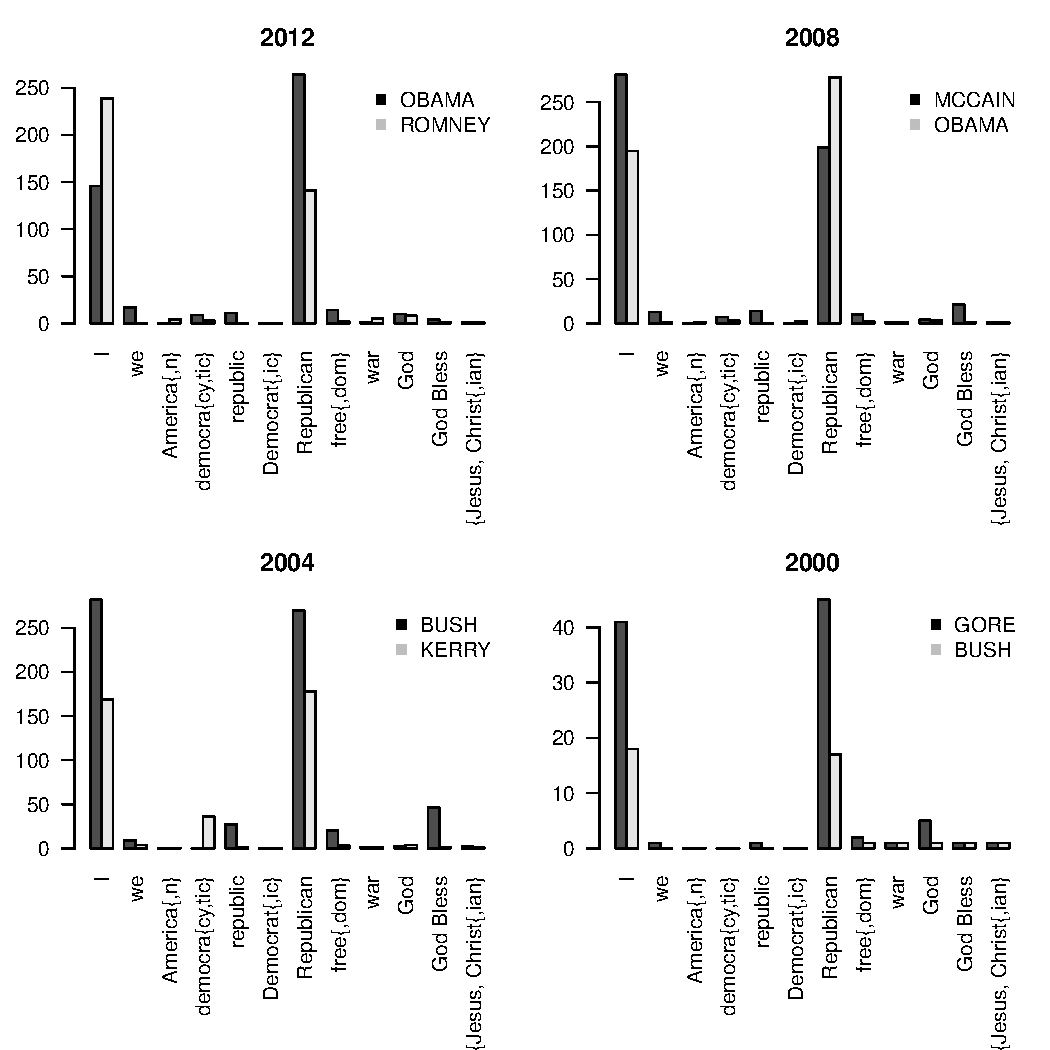
\includegraphics[width=\maxwidth]{figure/unnamed-chunk-17-1} 

\end{knitrout}
Looking at the histograms, we can say that Obama uses the word "I" less times than his Republican opponents. But surprisingly, Obama uses the word "Republican" more times than the Republicans themselves. This can highlights the fact that during the debates, he spent a lot of time criticizing his oppenent.
%%%%%%%%%%%%%%%%%%%%%%%%%%%%%%%%%%%%
\section{Problem 3}
%%%%%%%%%%%%%%%%%%%%%%%%%%%%%%%%%%%%
%%%%%%%%%%%%
\subsection{Random Walk}
%%%%%%%%%%%%
In order to compute the random walk I use the function rbinom which is useful for having a sequence of bernouilli variables 0,1. Then, I map the 0,1 output in order to have -1,1. Since the x and y variables are independent, we can split the walk for the x coordinate and the y coordinate, and then plot the corresponding path.\\
As an example, I compute a 100 steps Random Walk, return the final node and plot the corresponding path. The function takes into argument :
\begin{itemize}
\item n (integer) : number of steps in the random walk
\item out (string, default = "") : whether the function returns the path ("path") or only the final node ("last")
\item plot (bool, default = TRUE) : whether a plot of the path is displayed or not
\item origin (numeric, default = (0,0)) : origin of the random walk
\item legend (character, default = "bottomright") : localisation of the legend on the plot
\end{itemize}
Moreover, I create 3 exceptions to prevent the user that :
\begin{itemize}
\item n is not a number
\item n is not an integer number
\item n is not a positive integer
\end{itemize}
\begin{knitrout}
\definecolor{shadecolor}{rgb}{0.969, 0.969, 0.969}\color{fgcolor}\begin{kframe}
\begin{alltt}
\hlstd{random_walk} \hlkwb{=} \hlkwa{function} \hlstd{(}\hlkwc{n}\hlstd{,}\hlkwc{out}\hlstd{=}\hlstr{""}\hlstd{,}\hlkwc{plot}\hlstd{=T,}\hlkwc{origin}\hlstd{=}\hlkwd{c}\hlstd{(}\hlnum{0}\hlstd{,}\hlnum{0}\hlstd{),}
                        \hlkwc{legend}\hlstd{=}\hlstr{"bottomright"}\hlstd{)\{}
  \hlkwa{if} \hlstd{(}\hlopt{!}\hlkwd{is.numeric}\hlstd{(n))\{}
    \hlkwd{stop}\hlstd{(}\hlstr{"\textbackslash{}"n\textbackslash{}" is not a number"}\hlstd{)}
  \hlstd{\}}
  \hlkwa{else if} \hlstd{(}\hlopt{!}\hlstd{(}\hlkwd{floor}\hlstd{(n)}\hlopt{==}\hlstd{n))\{}
    \hlkwd{stop}\hlstd{(}\hlstr{"\textbackslash{}"n\textbackslash{}" is not an integer"}\hlstd{)}
  \hlstd{\}}
  \hlkwa{else if} \hlstd{(}\hlopt{!}\hlstd{(n}\hlopt{>}\hlnum{0}\hlstd{))\{}
    \hlkwd{stop}\hlstd{(}\hlstr{"\textbackslash{}"n\textbackslash{}" is not positive"}\hlstd{)}
  \hlstd{\}}
  \hlkwa{else}\hlstd{\{}
    \hlstd{x}\hlkwb{=}\hlkwd{c}\hlstd{(}\hlnum{0}\hlstd{,}\hlkwd{cumsum}\hlstd{(}\hlkwd{rbinom}\hlstd{(n,}\hlnum{1}\hlstd{,}\hlnum{0.5}\hlstd{)}\hlopt{-}\hlnum{0.5}\hlstd{)}\hlopt{*}\hlnum{2}\hlstd{)}\hlopt{+}\hlstd{origin[}\hlnum{1}\hlstd{]}
    \hlstd{y}\hlkwb{=}\hlkwd{c}\hlstd{(}\hlnum{0}\hlstd{,}\hlkwd{cumsum}\hlstd{(}\hlkwd{rbinom}\hlstd{(n,}\hlnum{1}\hlstd{,}\hlnum{0.5}\hlstd{)}\hlopt{-}\hlnum{0.5}\hlstd{)}\hlopt{*}\hlnum{2}\hlstd{)}\hlopt{+}\hlstd{origin[}\hlnum{2}\hlstd{]}
    \hlcom{#Plotting Options}
    \hlkwa{if} \hlstd{(plot)\{}
      \hlstd{ymax}\hlkwb{=}\hlkwd{max}\hlstd{(y)}
      \hlstd{ymin}\hlkwb{=}\hlkwd{min}\hlstd{(y)}
      \hlstd{xmax}\hlkwb{=}\hlkwd{max}\hlstd{(x)}
      \hlstd{xmin}\hlkwb{=}\hlkwd{min}\hlstd{(x)}
      \hlkwd{plot}\hlstd{(x,y,}\hlkwc{ylim}\hlstd{=}\hlkwd{c}\hlstd{(ymin,ymax),}\hlkwc{xlim}\hlstd{=}\hlkwd{c}\hlstd{(xmin,xmax),}\hlkwc{type}\hlstd{=}\hlstr{"b"}\hlstd{,}
           \hlkwc{cex}\hlstd{=}\hlkwd{rev}\hlstd{(}\hlkwd{seq}\hlstd{(}\hlnum{.5}\hlstd{,}\hlnum{2}\hlstd{,}\hlnum{1.5}\hlopt{/}\hlstd{n)),}\hlkwc{col}\hlstd{=}\hlkwd{gray}\hlstd{(}\hlkwd{rev}\hlstd{(}\hlkwd{seq}\hlstd{(}\hlnum{0}\hlstd{,}\hlnum{0.5}\hlstd{,}\hlnum{0.5}\hlopt{/}\hlstd{n)))}
           \hlstd{,}\hlkwc{pch}\hlstd{=}\hlnum{19}\hlstd{,}\hlkwc{main}\hlstd{=}\hlkwd{cat}\hlstd{(}\hlstr{"Random Walk, "}\hlstd{, n,} \hlstr{" steps"}\hlstd{))}
      \hlkwd{segments}\hlstd{(x[}\hlnum{1}\hlopt{:}\hlstd{(n}\hlopt{-}\hlnum{1}\hlstd{)],y[}\hlnum{1}\hlopt{:}\hlstd{(n}\hlopt{-}\hlnum{1}\hlstd{)],x[}\hlnum{2}\hlopt{:}\hlstd{n],y[}\hlnum{2}\hlopt{:}\hlstd{n],}\hlkwc{lwd}\hlstd{=}\hlnum{0.8}\hlstd{)}
      \hlkwd{points}\hlstd{(x[}\hlnum{1}\hlstd{],y[}\hlnum{1}\hlstd{],}\hlkwc{pch}\hlstd{=}\hlnum{9}\hlstd{,}\hlkwc{cex}\hlstd{=}\hlnum{3}\hlstd{)}
      \hlkwd{points}\hlstd{(x[n}\hlopt{+}\hlnum{1}\hlstd{],y[n}\hlopt{+}\hlnum{1}\hlstd{],}\hlkwc{pch}\hlstd{=}\hlnum{3}\hlstd{,}\hlkwc{cex}\hlstd{=}\hlnum{6}\hlstd{)}
      \hlkwd{legend}\hlstd{(} \hlkwc{x}\hlstd{=legend,}
            \hlkwc{legend}\hlstd{=}\hlkwd{c}\hlstd{(}\hlstr{"Initial Position"}\hlstd{,}\hlstr{"Final Position"}\hlstd{),}
            \hlkwc{pch}\hlstd{=}\hlkwd{c}\hlstd{(}\hlnum{9}\hlstd{,}\hlnum{3}\hlstd{) )}
    \hlstd{\}}
    \hlcom{#Return the path of the random walk}
    \hlkwa{if} \hlstd{(out}\hlopt{==}\hlstr{"path"}\hlstd{)}
      \hlkwd{return}\hlstd{(}\hlkwd{cbind}\hlstd{(x,y))}
    \hlcom{#Return the last position of the random walk olny}
    \hlkwa{if} \hlstd{(out} \hlopt{==} \hlstr{"last"}\hlstd{)}
      \hlkwd{return}\hlstd{(}\hlkwd{c}\hlstd{(x[n}\hlopt{+}\hlnum{1}\hlstd{],y[n}\hlopt{+}\hlnum{1}\hlstd{]))}
  \hlstd{\}}

\hlstd{\}}
\end{alltt}
\end{kframe}
\end{knitrout}
As an example, I plot a random walk with 100 steps and origin (0,0).
\begin{knitrout}
\definecolor{shadecolor}{rgb}{0.969, 0.969, 0.969}\color{fgcolor}\begin{kframe}
\begin{alltt}
\hlkwd{set.seed}\hlstd{(}\hlnum{15}\hlstd{)}
\hlkwd{random_walk}\hlstd{(}\hlnum{100}\hlstd{)}
\end{alltt}
\end{kframe}
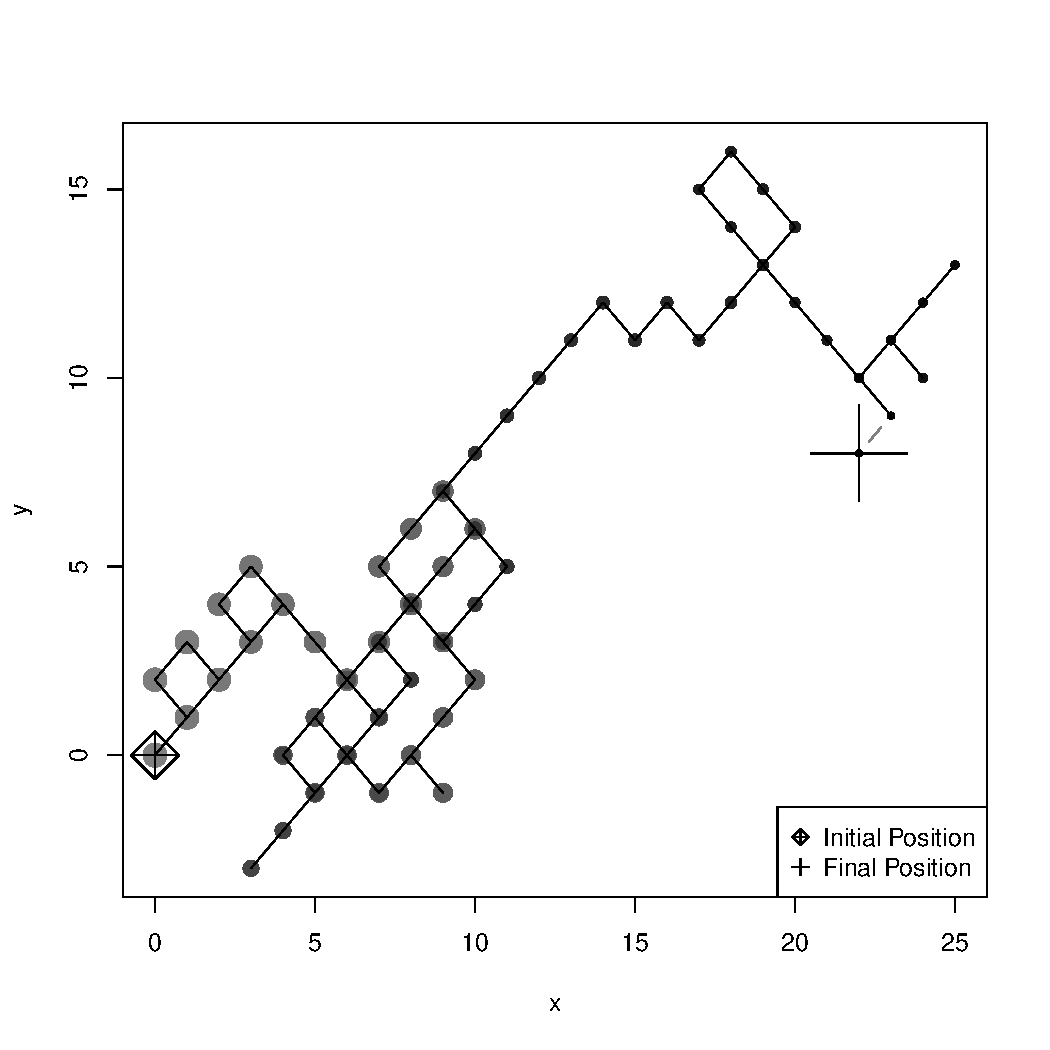
\includegraphics[width=\maxwidth]{figure/unnamed-chunk-19-1} 
\begin{kframe}\begin{lstlisting}[basicstyle=\ttfamily,breaklines=true]
## Random Walk,  100  steps
\end{lstlisting}
\end{kframe}
\end{knitrout}
For 10,000 steps, it looks like this :
\begin{knitrout}
\definecolor{shadecolor}{rgb}{0.969, 0.969, 0.969}\color{fgcolor}\begin{kframe}
\begin{alltt}
\hlkwd{set.seed}\hlstd{(}\hlnum{11}\hlstd{)}
\hlkwd{random_walk}\hlstd{(}\hlnum{10000}\hlstd{)}
\end{alltt}
\end{kframe}
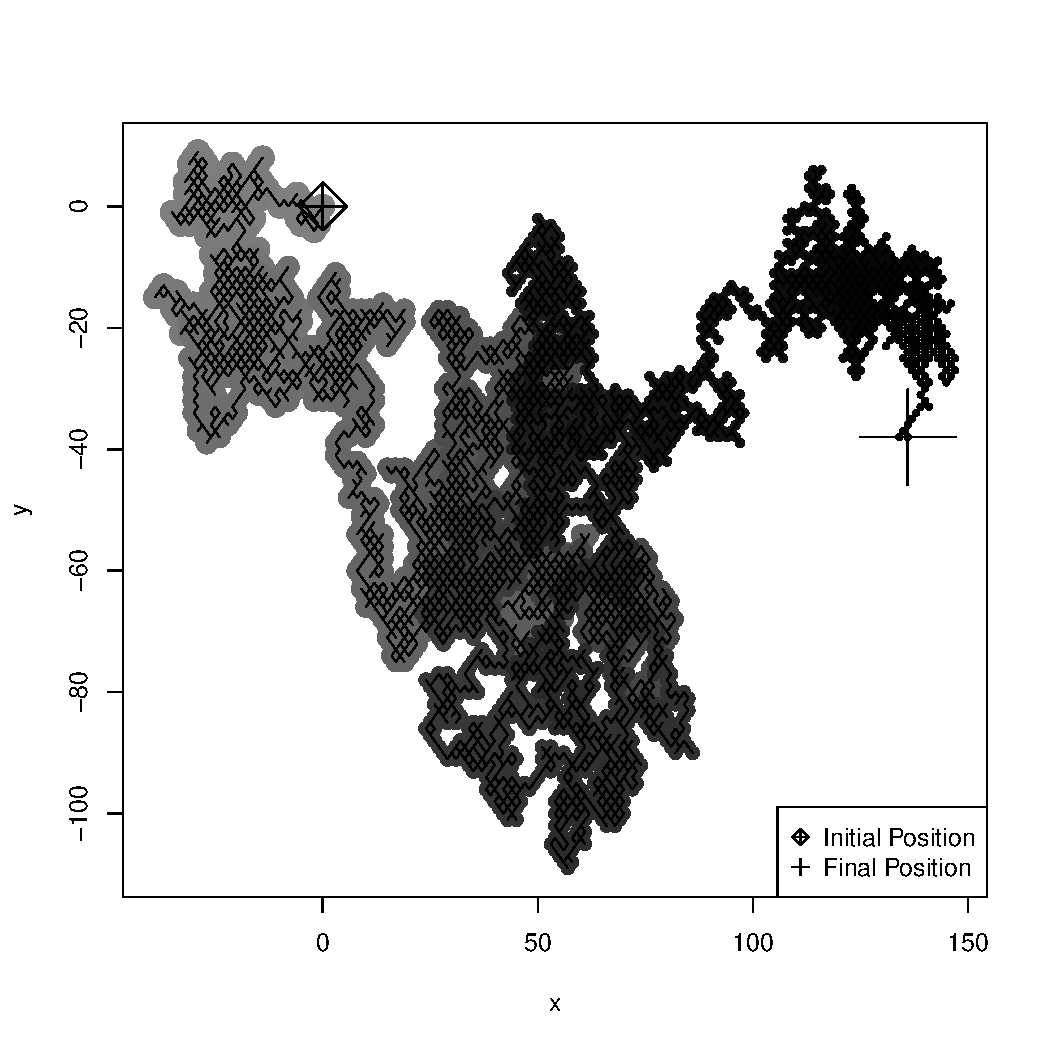
\includegraphics[width=\maxwidth]{figure/unnamed-chunk-20-1} 
\begin{kframe}\begin{lstlisting}[basicstyle=\ttfamily,breaklines=true]
## Random Walk,  10000  steps
\end{lstlisting}
\end{kframe}
\end{knitrout}
I can plot the path of the walk for an origin (4,5) :
\begin{knitrout}
\definecolor{shadecolor}{rgb}{0.969, 0.969, 0.969}\color{fgcolor}\begin{kframe}
\begin{alltt}
\hlkwd{set.seed}\hlstd{(}\hlnum{1}\hlstd{)}
\hlkwd{random_walk}\hlstd{(}\hlnum{10}\hlstd{,}\hlkwc{out}\hlstd{=}\hlstr{"path"}\hlstd{,}\hlkwc{origin}\hlstd{=}\hlkwd{c}\hlstd{(}\hlnum{4}\hlstd{,}\hlnum{5}\hlstd{),}\hlkwc{plot}\hlstd{=F)}
\end{alltt}
\begin{lstlisting}[basicstyle=\ttfamily,breaklines=true]
##       x y
##  [1,] 4 5
##  [2,] 3 4
##  [3,] 2 3
##  [4,] 3 4
##  [5,] 4 3
##  [6,] 3 4
##  [7,] 4 3
##  [8,] 5 4
##  [9,] 6 5
## [10,] 7 4
## [11,] 6 5
\end{lstlisting}
\end{kframe}
\end{knitrout}

%%%%%%%%%%%%
\subsection{S3 Classes}
I construct my rw class and the requested methods. In the constructor, I define two parameters : the number of steps of the random walk and the origin of it with a default value (0,0)
%%%%%%%%%%%%
\begin{knitrout}
\definecolor{shadecolor}{rgb}{0.969, 0.969, 0.969}\color{fgcolor}\begin{kframe}
\begin{alltt}
\hlcom{## @knitr constructor}
\hlstd{rw} \hlkwb{<-} \hlkwa{function}\hlstd{(}\hlkwc{steps}\hlstd{=}\hlnum{NA}\hlstd{,}\hlkwc{origin}\hlstd{=}\hlkwd{c}\hlstd{(}\hlnum{0}\hlstd{,}\hlnum{0}\hlstd{))\{}
  \hlcom{# constructor for 'indiv' class}
  \hlstd{obj} \hlkwb{<-} \hlkwd{list}\hlstd{(}\hlkwc{steps}\hlstd{=steps,}\hlkwc{origin}\hlstd{=origin)}
  \hlkwd{class}\hlstd{(obj)} \hlkwb{<-} \hlstr{'rw'}
  \hlkwd{return}\hlstd{(obj)}
\hlstd{\}}
\end{alltt}
\end{kframe}
\end{knitrout}
\begin{knitrout}
\definecolor{shadecolor}{rgb}{0.969, 0.969, 0.969}\color{fgcolor}\begin{kframe}
\begin{alltt}
\hlcom{## @knitr methods}
\hlstd{print.rw} \hlkwb{<-} \hlkwa{function}\hlstd{(}\hlkwc{object}\hlstd{)}
  \hlkwd{return}\hlstd{(}\hlkwd{random_walk}\hlstd{(object}\hlopt{$}\hlstd{steps,}\hlkwc{plot}\hlstd{=F,}\hlkwc{out}\hlstd{=}\hlstr{"last"}\hlstd{,}
                     \hlkwc{origin}\hlstd{=object}\hlopt{$}\hlstd{origin))}
\hlstd{plot.rw} \hlkwb{<-} \hlkwa{function}\hlstd{(}\hlkwc{object}\hlstd{,}\hlkwc{legend}\hlstd{=}\hlstr{"bottomright"}\hlstd{)}
  \hlkwd{return}\hlstd{(}\hlkwd{random_walk}\hlstd{(object}\hlopt{$}\hlstd{steps,}\hlkwc{plot}\hlstd{=T,}\hlkwc{out}\hlstd{=}\hlstr{""}\hlstd{,}\hlkwc{origin}\hlstd{=object}\hlopt{$}\hlstd{origin,}
                     \hlkwc{legend}\hlstd{=legend))}
\hlstd{summarize.rw} \hlkwb{<-} \hlkwa{function}\hlstd{(}\hlkwc{object}\hlstd{)}
  \hlkwd{return}\hlstd{(}\hlkwd{with}\hlstd{(object,} \hlkwd{cat}\hlstd{(}\hlstr{"Random walk with "}\hlstd{, steps,}
                          \hlstr{" steps and origin ("}\hlstd{, origin[}\hlnum{1}\hlstd{],}\hlstr{","}\hlstd{,}
                          \hlstd{origin[}\hlnum{2}\hlstd{],}\hlstr{").\textbackslash{}n"}\hlstd{,}\hlkwc{sep} \hlstd{=} \hlstr{""}\hlstd{)))}
\end{alltt}
\end{kframe}
\end{knitrout}
\begin{knitrout}
\definecolor{shadecolor}{rgb}{0.969, 0.969, 0.969}\color{fgcolor}\begin{kframe}
\begin{alltt}
\hlcom{## @knitr class-operators}
\hlstd{`[.rw`} \hlkwb{<-} \hlkwa{function}\hlstd{(}\hlkwc{object}\hlstd{,}\hlkwc{i}\hlstd{) \{}
  \hlstd{r}\hlkwb{=}\hlkwd{random_walk}\hlstd{(object}\hlopt{$}\hlstd{steps,}\hlkwc{origin}\hlstd{=object}\hlopt{$}\hlstd{origin,}\hlkwc{plot}\hlstd{=F,}\hlkwc{out}\hlstd{=}\hlstr{"path"}\hlstd{)}
  \hlkwd{return}\hlstd{(r[i}\hlopt{+}\hlnum{1}\hlstd{,])}
\hlstd{\}}
\end{alltt}
\end{kframe}
\end{knitrout}
\begin{knitrout}
\definecolor{shadecolor}{rgb}{0.969, 0.969, 0.969}\color{fgcolor}\begin{kframe}
\begin{alltt}
\hlcom{## @knitr replacement}
\hlstd{`start<-`} \hlkwb{<-} \hlkwa{function}\hlstd{(}\hlkwc{x}\hlstd{,} \hlkwc{...}\hlstd{)} \hlkwd{UseMethod}\hlstd{(}\hlstr{"start<-"}\hlstd{)}
\hlstd{`start<-.rw`} \hlkwb{<-} \hlkwa{function}\hlstd{(}\hlkwc{object}\hlstd{,} \hlkwc{value}\hlstd{)\{}
  \hlstd{object}\hlopt{$}\hlstd{origin} \hlkwb{<-} \hlstd{value}
  \hlkwd{return}\hlstd{(object)}
\hlstd{\}}
\end{alltt}
\end{kframe}
\end{knitrout}
Once I have defined my rw class, I can :
\begin{itemize}
\item Set a new "rw" variable called "walk".
\begin{knitrout}
\definecolor{shadecolor}{rgb}{0.969, 0.969, 0.969}\color{fgcolor}\begin{kframe}
\begin{alltt}
\hlkwd{set.seed}\hlstd{(}\hlnum{1}\hlstd{)}
\hlstd{walk} \hlkwb{<-} \hlkwd{rw}\hlstd{(}\hlnum{20}\hlstd{)}
\end{alltt}
\end{kframe}
\end{knitrout}

\item Redefine the start of the random walk.
\begin{knitrout}
\definecolor{shadecolor}{rgb}{0.969, 0.969, 0.969}\color{fgcolor}\begin{kframe}
\begin{alltt}
\hlkwd{start}\hlstd{(walk)} \hlkwb{=} \hlkwd{c}\hlstd{(}\hlnum{5}\hlstd{,} \hlnum{7}\hlstd{)}
\end{alltt}
\end{kframe}
\end{knitrout}
\item Print the summary of the walk object.
\begin{knitrout}
\definecolor{shadecolor}{rgb}{0.969, 0.969, 0.969}\color{fgcolor}\begin{kframe}
\begin{alltt}
\hlkwd{summarize.rw}\hlstd{(walk)}
\end{alltt}
\begin{lstlisting}[basicstyle=\ttfamily,breaklines=true]
## Random walk with 20 steps and origin (5,7).
\end{lstlisting}
\end{kframe}
\end{knitrout}
\item Return the third position of the random walk.
\begin{knitrout}
\definecolor{shadecolor}{rgb}{0.969, 0.969, 0.969}\color{fgcolor}\begin{kframe}
\begin{alltt}
\hlkwd{`[`}\hlstd{(walk,}\hlnum{3}\hlstd{)}
\end{alltt}
\begin{lstlisting}[basicstyle=\ttfamily,breaklines=true]
## x y 
## 4 8
\end{lstlisting}
\end{kframe}
\end{knitrout}
\item Plot the walk using the new plot method for rw objects.
\begin{knitrout}
\definecolor{shadecolor}{rgb}{0.969, 0.969, 0.969}\color{fgcolor}\begin{kframe}
\begin{alltt}
\hlkwd{plot}\hlstd{(walk,}\hlkwc{legend}\hlstd{=}\hlstr{"topright"}\hlstd{)}
\end{alltt}
\end{kframe}
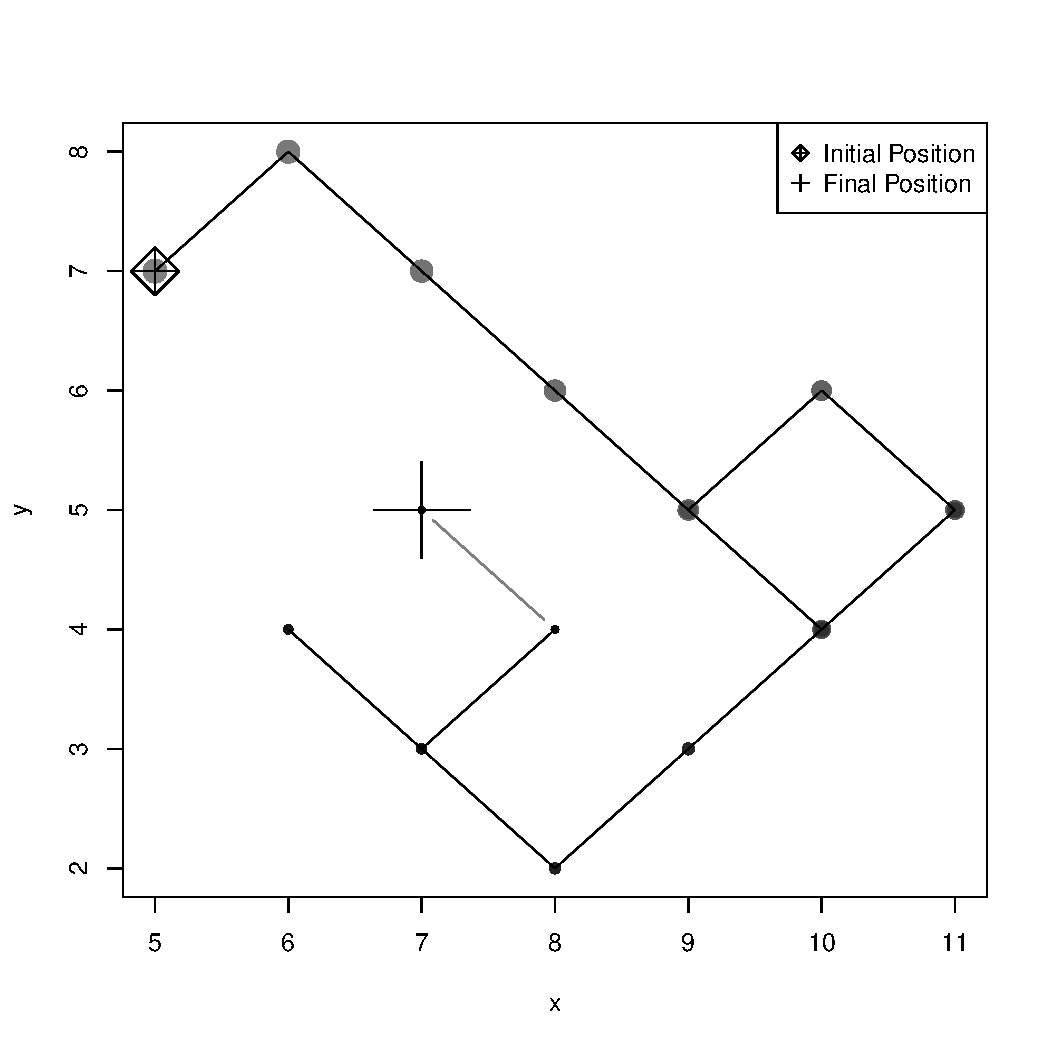
\includegraphics[width=\maxwidth]{figure/unnamed-chunk-30-1} 
\begin{kframe}\begin{lstlisting}[basicstyle=\ttfamily,breaklines=true]
## Random Walk,  20  steps
\end{lstlisting}
\end{kframe}
\end{knitrout}
\end{itemize}

\end{document}
